% Chapter Template

\chapter{Implementation} % Main chapter title

\label{Chapter4} % Change X to a consecutive number; for referencing this chapter elsewhere, use \ref{ChapterX}

%----------------------------------------------------------------------------------------
%	SECTION 1
%----------------------------------------------------------------------------------------

\section{Overview}
Most of the implementation apart from the custom neuron and synapse models is written in Python 3.9. This offers the opportunity to create an object-oriented implementation, loosely inspired by the original work of \parencite{klampfl_maass_2013}. The fundamental object classes this project uses are:
\begin{itemize}
    \item \texttt{WTACircuit}: Serves as the basic component to organize sets of neurons that are supposed to form the same WTA circuit. (Section \ref{sec:wta_circuit_network})
    \item \texttt{Network}: The centerpiece of this project, implementing the grid composition of \texttt{WTACircuit} objects as well as the inter-network neuron connections. (Section \ref{sec:wta_circuit_network})
    \item \texttt{InputGenerator}: Responsible for the setup and tuning of pattern and noise input to the network during simulation. (Section \ref{sec:input_generation})
    \item \texttt{Recorder}: Manages the simulation of the associated \texttt{InputGenerator} and \texttt{Network} as well as the recording of Network properties like spiking input, network spike behavior, membrane potential, EPSP, and weight. Also responsible for plotting the recorded data. (Section \ref{sec:recording})
\end{itemize}
These object classes can be seen in Figure \ref{fig:implementation_concept_drawing} where their relation to each other, structure, and function is conceptually illustrated. It is important to point out, however, that the Python part of this project is only responsible for the organization, creation, and manipulation of NEST components like neurons, synapses, spike generators, and measurement devices. Most of the heavy lifting in the background required to operate and simulate these is outsourced to NEST. The source code for this thesis can be found in \parencite{michau_2022}.
\begin{figure}[htbp]
    \centering
    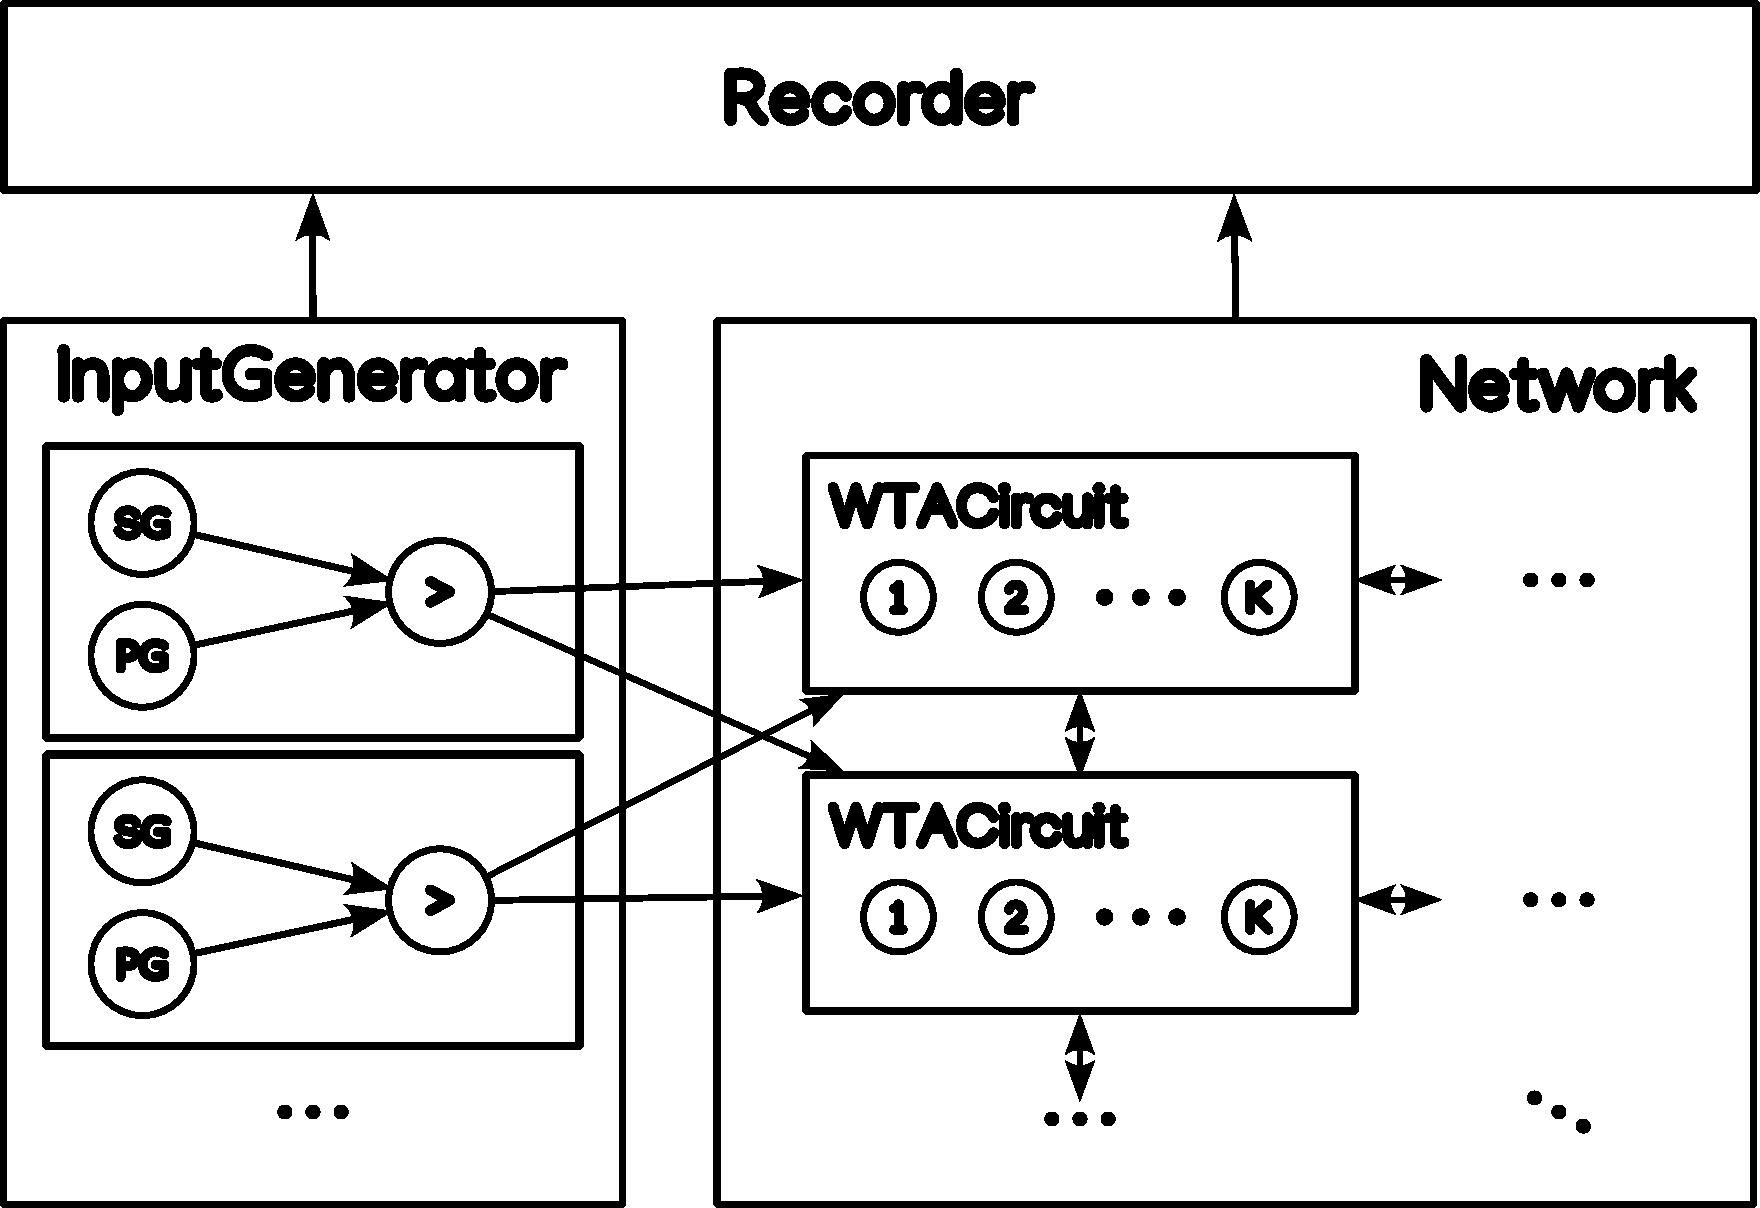
\includegraphics[width=\columnwidth]{Figures/implementation_conceptual.pdf}
    \caption{Conceptual Drawing of Implementation. Definition of terms: \textbf{SG} denotes 'Spikegenerator', \textbf{PG} denotes 'Poissongenerator' and \textbf{>} denotes 'Parrot neuron'.}
    \label{fig:implementation_concept_drawing}
\end{figure}

% name basic components and underlying design principle of the implementation
% describe basic functionality of nest/NESTML
\section{WTA Circuit Network} \label{sec:wta_circuit_network}
\subsection{Grid}
To model the distance-dependent connection probability described in Equation \ref{eqn:distance_dependent_probability} it is necessary to first assign each neuron in the network a spatial coordinate to determine the distance between different WTA circuits. While NEST provides the possibility to construct spatially structured spiking neural networks, together with a range of supporting functionality that is needed to replicate the model from \parencite{klampfl_maass_2013}, some details stand in the way of their use. First and foremost, the NEST spatially structured networks are designed to be biologically plausible, i.e. work in three dimensions, as do all their functionalities like e.g. functions to determine distances. Meanwhile, the \parencite{klampfl_maass_2013} model is rather implemented using a 2D grid where the coordinates are assigned on a per WTA basis, leading to multiple neurons having the same coordinates. As this would be difficult to implement in NEST, a simpler approach was pursued instead.\\
Instead of using NEST's spatially structured network functionality, a custom \texttt{WTACircuit} object (Figure \ref{fig:object_wta_circuit}) was introduced, featuring a 2D-coordinate \texttt{pos} indicating the position on the grid and a NodeCollection of size \texttt{k}:\\
\begin{figure}[htbp]
\centering
\begin{tikzpicture}
\begin{class}[text width=0.9\columnwidth]{WTACircuit}{0,0}
    \attribute{nc : \textbf{NodeCollection}}
    \attribute{pos : \textbf{tuple}}
    \attribute{k : \textbf{int}}
    \operation{\_\_init\_\_(nc: \textbf{NodeCollection}, pos: \textbf{tuple})}
    \operation{form\_WTA() $\rightarrow$ \textbf{NoneType}}
    \operation{get\_pos() $\rightarrow$ \textbf{tuple}}
    \operation{get\_x() $\rightarrow$ \textbf{int}}
    \operation{get\_y() $\rightarrow$ \textbf{int}}
    \operation{get\_node\_collection() $\rightarrow$ \textbf{NodeCollection}}
    \operation{get\_size() $\rightarrow$ \textbf{int}}
\end{class}
\end{tikzpicture}
\caption{\texttt{WTACircuit} Class Diagram} \label{fig:object_wta_circuit}
\end{figure}
\\
As can be seen from Figure \ref{fig:object_wta_circuit}, the \texttt{WTACircuit} object is initialized using a position tuple and a NodeCollection. This NodeCollection type is how NEST handles neurons of any kind that have been previously created. The initialization function \texttt{\_\_init\_\_()} also instantiates \texttt{k} with the size of the NodeCollection \texttt{nc} using \texttt{get\_size()} and most notably connects every neuron in \texttt{nc} to every other neuron via an InstantaneousRateConnection. These connections do not model any synapses and are in fact a makeshift solution that had to be manually implemented to the neuron model in C++ because they are necessary for the abstract implementation of lateral inhibition without dedicated inhibitory neurons as stated by \parencite{klampfl_maass_2013}, which is not provided by NEST or NESTML.
These InstantaneousRateConnections were originally developed in NEST for use in continuous rate models, where they would communicate rates. For this thesis, they were modified to enable the communication of membrane potentials within the WTA circuit. This is crucial for the calculation of the firing rate (Equation \ref{eqn:firing_rate_paper}) since each node has to calculate it on its own and is therefore dependent on the firing rates of its fellow neurons in the WTA.
\begin{figure}[htbp]
\centering
\begin{tikzpicture}
\begin{class}[text width=0.9\columnwidth]{Network}{0,0}
    \attribute{grid\_shape: \textbf{tuple}}
    \attribute{n: \textbf{int}}
    \attribute{m: \textbf{int}}
    \attribute{k\_min: \textbf{int}}
    \attribute{k\_max: \textbf{int}}
    \attribute{n\_inputs: \textbf{int}}
    \attribute{lam: \textbf{float}}
    \attribute{circuits: \textbf{list}}
    \attribute{save\_figures: \textbf{bool}}
    \attribute{show\_figures: \textbf{bool}}
    \operation{\_\_init\_\_(**kwds)}
    \operation{create\_grid() $\rightarrow$ \textbf{list}}
    \operation{form\_connections() $\rightarrow$ \textbf{NoneType}}
    \operation{get\_circuit\_grid() $\rightarrow$ \textbf{numpy.ndarray}}
    \operation{get\_node\_collections(slice\_min: \textbf{int}, slice\_max: \textbf{int}) $\rightarrow$ \textbf{NodeCollection}}
    \operation{get\_pos\_by\_id() $\rightarrow$ \textbf{tuple}}
    \operation{visualize\_circuits() $\rightarrow$ \textbf{NoneType}}
\end{class}
\end{tikzpicture}
\caption{\texttt{Network} Class Diagram} \label{fig:object_network}
\end{figure}
\\ \ \\
The \texttt{Network} object in turn uses the \texttt{WTACircuit}s to construct a grid of shape $\texttt{n}\times\texttt{m}$ with them, where each \texttt{WTACircuit} has its size \texttt{K} uniformly drawn at random from the interval $[\texttt{k\_min}, \texttt{k\_max}]$. After the creation of the WTA grid using \texttt{create\_grid()}, all neurons in the network regardless of WTA association are connected to each other with probability derived from the distance-dependent probability rule from Equation \ref{eqn:distance_dependent_probability}. Additionally, the formation of \textit{autapses} (self-recurrent connections from the neuron to itself) are disabled. Initially, the synaptic weights of these connections are set to $1$, but they can also be randomized just as in \parencite{klampfl_maass_2013} by assigning the weights to $-\log(x)$, where $x\in[0; 1]$ is a random number.

\section{Input Generation} \label{sec:input_generation}
\begin{wrapfigure}{r}{0.45\textwidth}
    \begin{center}
        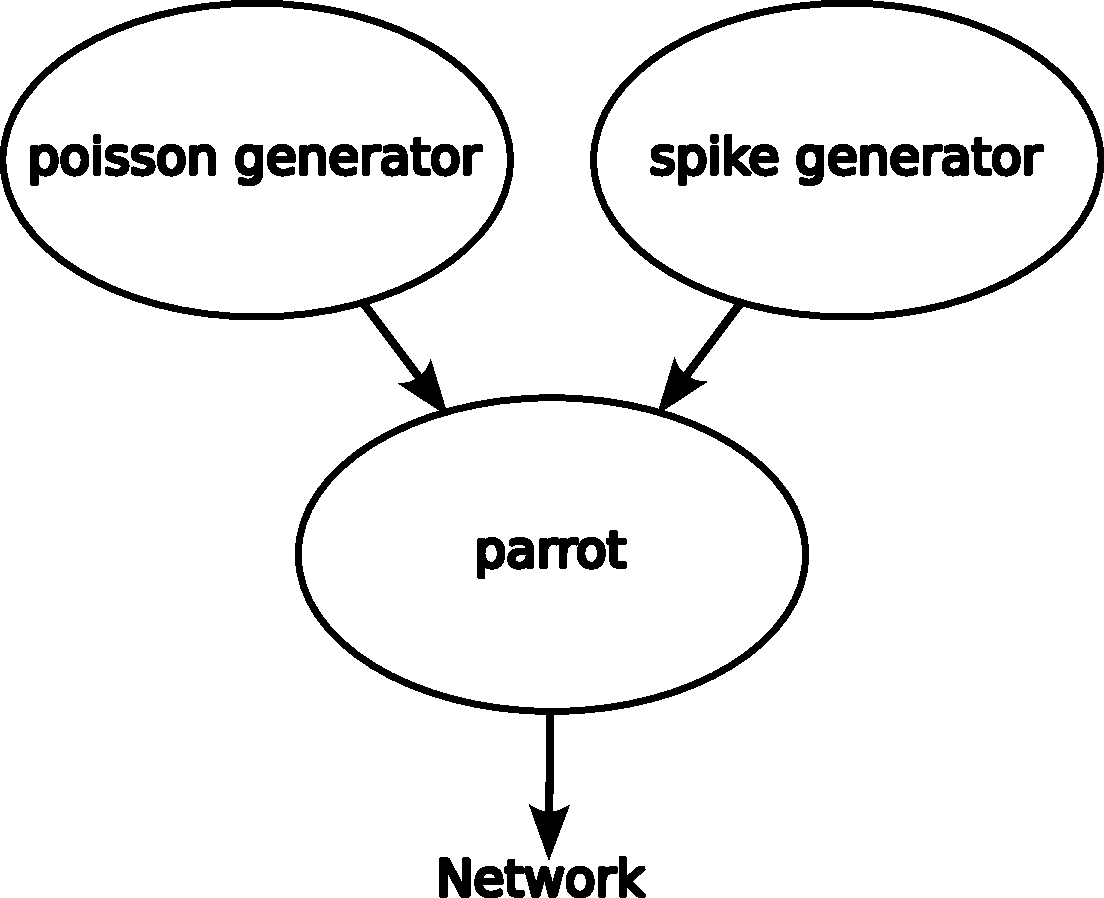
\includegraphics[width=0.4\columnwidth]{Figures/input_generator_structure.pdf}
    \end{center}
\caption{Single Input Assembly}
\label{fig:input_generator_structure}
\end{wrapfigure}
On the conceptual NEST level, each \texttt{InputGenerator} consists of \texttt{n} input assemblies as in Figure \ref{fig:input_generator_structure}. NESTs \textit{inhomogeneous\_poisson\_generator} is responsible for the creation of Poisson noise of specified rates for specified time intervals. The need for doing so is discussed later. 
Because a Poisson generator in NEST produces unique output for each neuron it is connected to - which is to be avoided to stay accurate to the original implementation - an additional \textit{parrot\_neuron} is interposed between the network and the Poisson generator. A parrot neuron in NEST just repeats the spikes it receives to all its connected targets, which effectively results in each network neuron receiving exactly the same noise input from the \textit{inhomogeneous\_poisson\_generator}.\\
The \textit{spike\_generator} handles the presentation of the pattern input as described in Chapter \ref{sec:input_generation}. Technically there is no need to connect it to a parrot, like the Poisson generator, but connecting it to the same parrot has the benefit that the input now enters the network over the same synapse. If the generator was connected to the network directly using its own synapse with plasticity, it is possible that the network might favor the pattern input over the noise by adjusting the synaptic weights, which would nullify the presence of noise in the first place. Also, this approach is more accurate to the original implementation.
\begin{figure}[htbp]
    \centering
    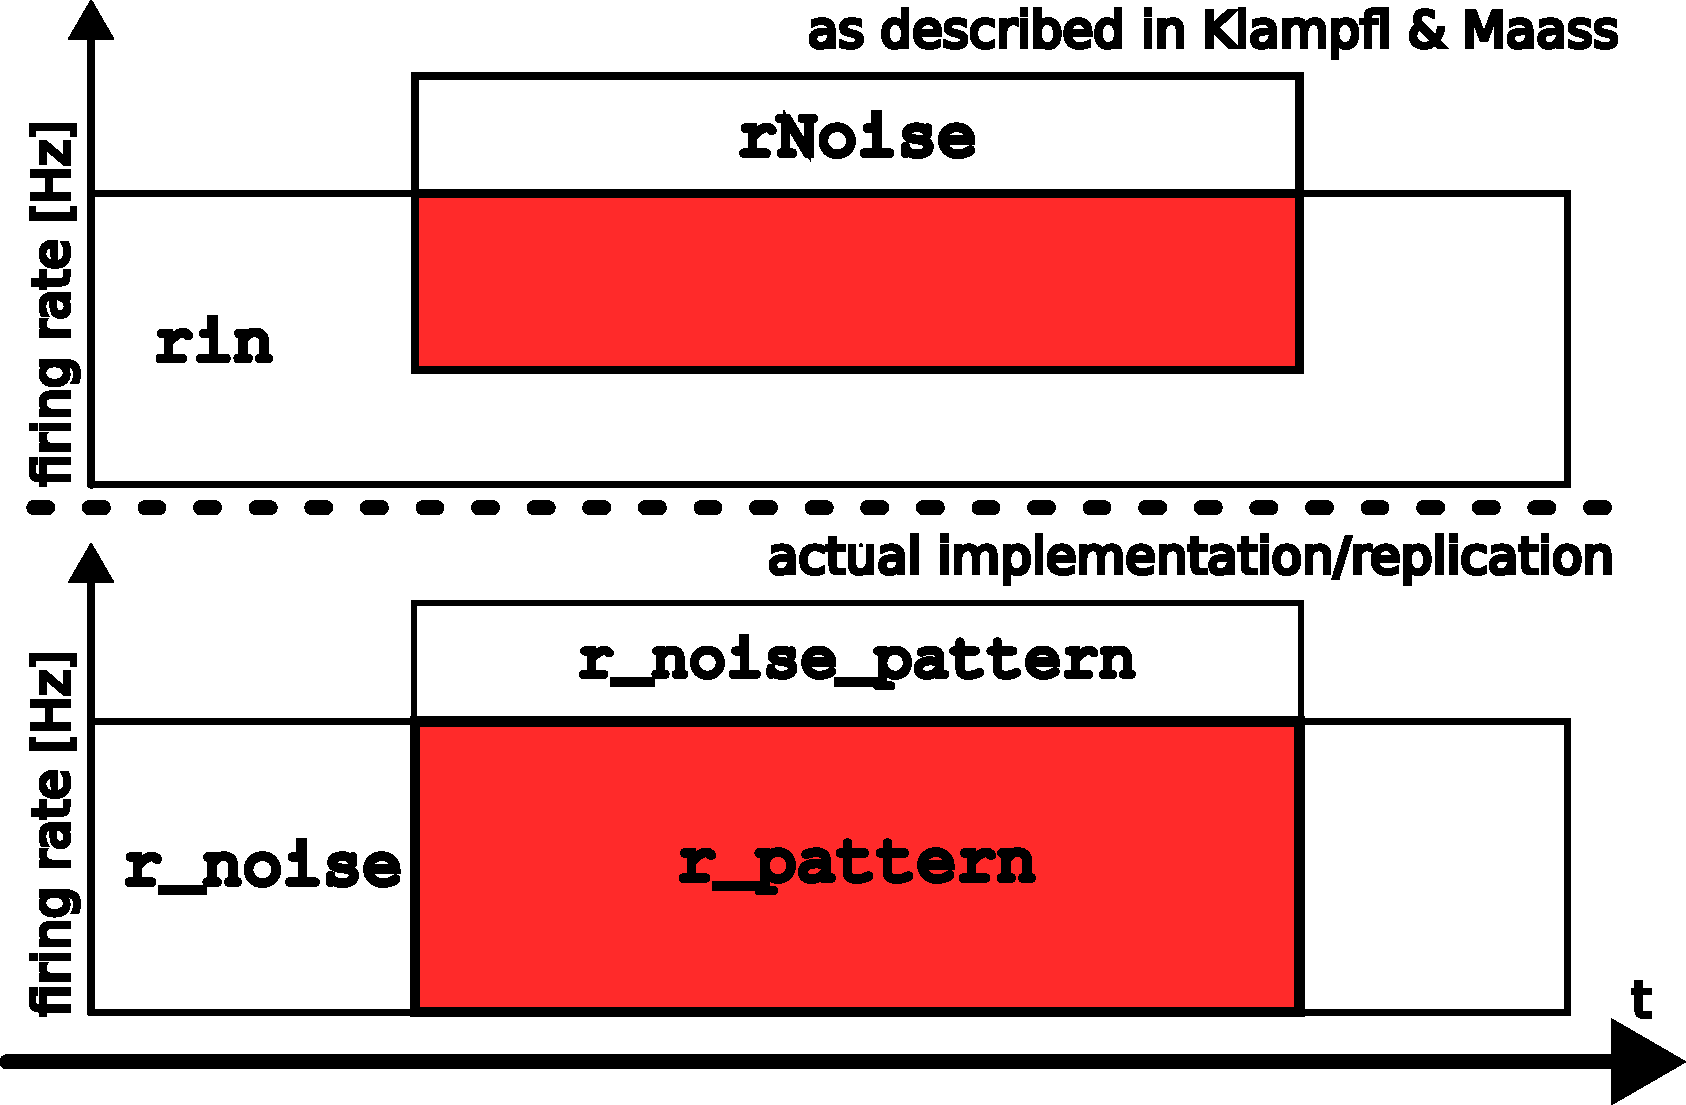
\includegraphics[width=0.9\columnwidth]{Figures/input_rates.pdf}
    \caption{Input rate comparison with pattern in red and noise in white}
    \label{fig:input_rates}
\end{figure}
\\
As mentioned earlier, different noise rates are needed for different time intervals. The reason for this is that unlike the distinction in "noise" and "pattern" phases might suggest, noise and pattern input are not mutually exclusive. In fact, pattern phases are usually superimposed with additional noise, requiring different noise rates during pattern presentation. There is however a difference between the reality of both the original and replicated implementation and the description from the paper as is illustrated in Figure \ref{fig:input_rates}. According to the description of Figure 4A in \parencite{klampfl_maass_2013}, a pattern of \SI{3}{\hertz} is embedded into an input spike train with constant rate \texttt{rin}=\SI{5}{\hertz} with additional \texttt{rNoise}=\SI{2}{\hertz} of noise laid over pattern presentations (Figure \ref{fig:input_rates} (top)). In the implementation of that same paper it was found however, that no embedding took place and the patterns had firing rate \SI{5}{\hertz}, just like \texttt{rin}.\\
The problem with the varying noise rates can be elegantly solved, since NEST provides a spike generator that offers a simple solution to this: the \textit{inhomogeneous\_poisson\_generator}. It generates Poisson noise of constant rate just like the regular \textit{poisson\_generator}, but in addition, allows for different noise rates at different intervals. This is used to specify two different noise rates: \texttt{r\_noise}, which is equivalent to \texttt{rin} during the noise phase, and \texttt{r\_noise\_pattern}, which is equivalent to the summed rate of \texttt{rNoise} and the noise remainder of \texttt{rin} during pattern presentation. This results in the same rate behavior and noise rate as in \parencite{klampfl_maass_2013}, while also taking advantage of NEST and simplifying the input generation.
\\ \ \\
With the groundwork of the \texttt{InputGenerator} described, the different possibilities for input generation and general procedure can be explained now with help from Figure \ref{fig:object_inputgenerator}. The general functioning of this is equivalent to the one described in Chapter \ref{sec:input_generation}. To tie in with the paragraph above, the different firing rates \texttt{r\_noise}, \texttt{r\_noise\_pattern}, \texttt{r\_input} can be freely set, as can be the number \texttt{n} of input channel assemblies from Figure \ref{fig:input_generator_structure}. It is however not required to play noise during simulation since it is determined by the value of \texttt{use\_noise}. To make the generator produce one or more input patterns or sequences of input patterns it has to be given the total number \texttt{n\_patterns} of different patterns it should create together with a duration for each of them in \texttt{t\_pattern}. These are created once by \texttt{create\_patterns()} and then stored for later use in \texttt{pattern\_list}.
The different sequences of patterns to present are contained \texttt{pattern\_sequences}, a list that specifies all possible compound sequences by the indices of patterns. A possible assignment for this could be [[0, 1], [2]], meaning that possible pattern combinations to present are pattern 0 directly followed by pattern 1 and pattern 2 alone. The order in which to present these sequences is determined by the sequence switching probability \texttt{p\_switch}, and \texttt{pattern\_mode}, which can be set to either of two modes \texttt{'random\_independent'} or \texttt{'random\_iterate'}. On \texttt{'random\_independent'} it selects the next sequence to present independently of previously played ones and on \texttt{'random\_iterate'} the next sequence from \texttt{pattern\_sequences} is presented with probability \texttt{p\_switch}, or the other way around, the current sequence is repeated with probability $1-$\texttt{p\_switch}.
\\ \ \\
The \texttt{InputGenerator} also stores information about the beginning of noise and pattern presentation phases that are used in the \texttt{Recorder} to order the spiking neuron output by mean activation time to make assemblies of neurons better recognizable. The data needed for this is stored in \texttt{phase\_times}, \texttt{pattern\_trace} and \texttt{next\_pattern\_length}.

\begin{figure}[htbp]
\centering
\begin{tikzpicture}
\begin{class}[text width=0.9\columnwidth]{InputGenerator}{0,0}
    \attribute{n: \textbf{int}}
    \attribute{target\_network: \textbf{NodeCollection}}
    \attribute{r\_noise: \textbf{int}}
    \attribute{r\_noise\_pattern: \textbf{int}}
    \attribute{r\_input: \textbf{int}}
    \attribute{n\_patterns: \textbf{int}}
    \attribute{pattern\_sequences: \textbf{list}}
    \attribute{pattern\_mode: \textbf{string}}
    \attribute{p\_switch: \textbf{float}}
    \attribute{t\_pattern: \textbf{list}}
    \attribute{t\_noise\_range: \textbf{list}}
    \attribute{pattern\_list: \textbf{list}}
    \attribute{spiketrain: \textbf{list}}
    \attribute{current\_pattern\_index: \textbf{list}}
    \attribute{spike\_generators: \textbf{NodeCollection}}
    \attribute{poisson\_generators: \textbf{NodeCollection}}
    \attribute{parrots: \textbf{NodeCollection}}
    \attribute{use\_noise: \textbf{bool}}
    \attribute{phase\_times: \textbf{list}}
    \attribute{pattern\_trace: \textbf{list}}
    \attribute{next\_pattern\_length: \textbf{list}}

    \operation{\_\_init\_\_(target\_network: \textbf{Network}, **kwargs) $\rightarrow$ \textbf{NoneType}}
    \operation{generate\_noise() $\rightarrow$ \textbf{NoneType}}
    \operation{create\_patterns() $\rightarrow$ \textbf{NoneType}}
    \operation{connect\_parrots() $\rightarrow$ \textbf{NoneType}}
    \operation{generate\_input(duration: \textbf{float}, t\_origin: \textbf{float}, force\_refresh\_patterns: \textbf{bool}) $\rightarrow$ \textbf{NoneType}}
    \operation{get\_next\_pattern\_id() $\rightarrow$ \textbf{int}}
    \operation{get\_patterns() $\rightarrow$ \textbf{list}}
    \operation{set\_patterns(patterns: \textbf{list}) $\rightarrow$ \textbf{NoneType}}
\end{class}
\end{tikzpicture}
\caption{\texttt{InputGenerator} Class Diagram} \label{fig:object_inputgenerator}
\end{figure}

%\begin{algorithm}
%	\caption{generate\_input(duration, t\_origin)} 
%	\begin{algorithmic}[1]
%	    \State t = 0
%	    \While{t < duration}
%	        \State t\_noise\_phase = random[t\_noise\_range]
%	        \For{ $i = 1,2,\dots, $n\_inputs}
%	            
%	        \EndFor
%	    \EndWhile
%	\end{algorithmic} 
%\end{algorithm}



\section{Recording and Measurement} \label{sec:recording}
\begin{figure}[htbp]
\centering
\begin{tikzpicture}
\begin{class}[text width=0.9\columnwidth]{Recorder}{0,0}
    \attribute{network: \textbf{Network}}
    \attribute{id\_list: \textbf{list}}
    \attribute{create\_plot: \textbf{bool}}
    \attribute{save\_figures: \textbf{bool}}
    \attribute{show\_figures: \textbf{bool}}
    \attribute{plot\_history: \textbf{bool}}
    \attribute{order\_neurons: \textbf{bool}}
    \attribute{dt\_rec : \textbf{int}}

    \operation{\_\_init\_\_(network: \textbf{Network}, id\_list: \textbf{list}, **kwargs)}
    \operation{set(**kwargs) $\rightarrow$ \textbf{NoneType}}
    \operation{run\_network() $\rightarrow$ \textbf{list}}
    \operation{record\_variables\_step() $\rightarrow$ \textbf{NoneType}}
    \operation{simulate(inpgen: \textbf{InputGenerator}, t: \textbf{int}, dt\_rec: \textbf{int}) $\rightarrow$ \textbf{NoneType}}
    \operation{get\_order(p: \textbf{list}, I: \textbf{list}, t: \textbf{list}, r\_fracs: \textbf{list}, tstart: \textbf{int}, nsteps: \textbf{int}) $\rightarrow$ \textbf{numpy.ndarray}}
\end{class}
\end{tikzpicture}
\caption{\texttt{Recorder} Class Diagram} \label{fig:object_recorder}
\end{figure}
The last object class on the Python level is the \texttt{Recorder}. While the other classes are mainly used for constructive work of the network, the \texttt{Recorder}s main function is to manage the simulation of that same network. For this it takes a \texttt{Network} object on construction with \texttt{\_\_init\_\_()}, along with an optional \texttt{id\_list} that contains the global IDs of the neurons from the \texttt{Network} that should be measured and plotted later as well as a set of self explanatory Boolean parameters (see Figure \ref{fig:object_recorder}) representing options for plotting outputs. Although these should be specified on initialization of a new \texttt{Recorder} object, all parameters can be changed later using the \texttt{set()} function. Since the \texttt{Recorder} handles simulation, the \texttt{run\_network()} function is its main function. It takes an \texttt{InputGenerator} (although this is optional) and simulates a network for a given period of time \texttt{t\_sim} with STDP/learning enabled or disabled, determined by the truth value of \texttt{train}. Because it is not always necessary or wanted to measure and plot the entire network, there are three different options besides recording the entire network:
\begin{enumerate}
    \item "Watch List": A list of neuron IDs \texttt{id\_list} to record from can be given to \texttt{run\_network()}. This is a good option for recording the same neurons over several network simulation sessions.
    \item "NodeCollection": A NodeCollection \texttt{node\_collection}, subset of the \texttt{Network} is specified and recorded.
    \item "Random $k$": $k$ neurons are randomly selected from the \texttt{Network} to record from. This is useful for creating a sample to record from in the very first simulation and then reusing the same sample in the "Watch List" mode.   
\end{enumerate} 
The general procedure of the \texttt{run\_network()} function starts by setting up recording devices, i.e. NEST \textit{multimeter} and \textit{spikerecorder} for the network and another separate \textit{spikerecorder} for the \texttt{InputGenerator}. The EPSPs and weights from the network are recorded by a separate \texttt{record\_variable\_step()} function by reading out network variables that were specifically made recordable to Python for this purpose in the C++ neuron model. Because reading out these variables does not work parallel to running the simulation, the simulation must be run in time steps of size \texttt{dt\_rec}. Setting this recording time window smaller will increase the resolution of the recording but comes with the trade-off of immensely deteriorated simulation efficiency and increased runtime.\\
After the setup of the recording devices, the actual simulation is run using the \texttt{simulate()} function that pre-generates the patterns of the \texttt{InputGenerator} for the duration of the simulation and then commands the NEST kernel to run the simulation for increments of \texttt{dt\_rec} and recording between increments until the NEST simulation has run for \texttt{t\_sim}. When the simulation and data collection are finished, the results are plotted. Optionally with neurons in the \textit{spikerecorder} readout ordered by their mean activation time during pattern presentation. This makes formed assemblies of neurons with related spiking behavior on input better visible.

\section{Neuron and Synapse Models} \label{sec:neuron_synapse_models}
As already mentioned in the Introduction, the models of the neuron and the synapse had to be implemented in C++ because NESTML did not provide the needed functionality. Before elaborating on the implementation, the concept of NEST synapse and neuron models needs to be explained. While in the original implementation all the neuron and synapse properties are handled in large arrays for the entirety of the network, in NEST each synapse and neuron is its own entity with a set of parameters. These entities are defined by models formulated in C++. Converting the original code into an object-oriented version proved to be very challenging and made it difficult to directly compare both implementations and detect errors. This will be covered in more detail in Chapter \ref{Chapter6}.

\subsection{Neurons} \label{ssec:neurons}
The custom neuron model follows a strict procedure to realize the same behavior as its non-object-oriented ancestor. The foundations of this procedure stem from NESTML \parencite{nestml_5_0_0}, although it was eventually abandoned as a modeling language. A neuron in NEST is generally updated on every simulation step, by the \texttt{update()} function, which first calls to \texttt{evolve\_epsps()} to update the current membrane potentials as described in Equations \ref{eqn:membrane_potential} and \ref{eqn:epsp}. Preceding that, input in the form of both \texttt{SpikeEvent}s and \texttt{InstantaneousRateConnectionEvent}s (described later) is managed by individual \texttt{handle()} functions. More precisely, on an incoming event of either kind, the properties of the spike are stored for later processing (e.g. by the \texttt{update()} function). 
\\ \ \\
%\subsubsection{Intermezzo: Operational Problems}
Implementing the membrane potential in NEST required a fair amount of creativity, given that Equation \ref{eqn:membrane_potential}, which defines it requires both the membrane potentials from all other neurons in the same WTA (although NEST neuron models have no concept of such things as WTAs) and the weights from all incoming synapses, which is not conventionally available from the postsynaptic neuron since it is a property of the synapse. These two problems made it entirely impossible to implement the model in NESTML, making the implementation even more complex and time-consuming, since the model now had to be manually written in C++ without the help of a modeling language, which was not intended when planning this thesis.\\
As already alluded to before, the problem of communicating the membrane potential (needed for calculating the summed firing rate of the WTA), was solved by introducing a new connection type already existing in NEST called \texttt{rate\_connection\_instantaneous}. Because it was originally designed for connecting rate model neurons it had to be modified to send and receive membrane potentials instead of firing rates. These connections are created \textit{all-to-all} (excluding self loops) between the neurons in the same WTA by the \texttt{form\_WTA} function on the Python level.\\
The second problem about the synapse weights was solved by creating a new internal vector \texttt{localWeights\_Wk} that was initialized with length $1000$ and filled with $0$ on construction. Setting the length fixed to $1000$ is not a perfect solution because this also means that for now, each neuron can only have as much as $1000$ presynaptic neurons and if it has less there may be a considerable overhead slowing down the simulation and wasting space. This can likely be fixed by using vectors of dynamic sizes and initializing them on network creation before the simulation starts. But since this was not a priority and did not cause problems for now, this remains to be implemented at a later point in time.
\\ \ \\
Following the calculation of membrane potential, \texttt{evolve\_epsps()} also updates the decay-time EPSP and rise-time EPSP from Equation \ref{eqn:epsp} using the update rule found in the original code (Equation \ref{eqn:epsp_update}). After the current membrane has been determined this way, the firing rate is set as defined in Equation \ref{eqn:firing_rate_paper}, with two additions. The first is that the term to calculate a neuron's fraction of firing rate in the WTA
\begin{equation*}
    \texttt{rate\_fraction}_k(t)=\frac{\exp(u_k(t))}{\sum_{j=1}^K\exp(u_j(t))}
\end{equation*}
is stored in a variable for use in the ordering function to later sort the neurons by mean activation time for better identifiability of output assemblies. The second is that the firing rate of the neuron is set to $0$ if the above rate fraction is larger than $1$. This should be impossible, but it has been found that due to an issue with the value initialization in NEST this can occur and tamper with the correct results. Setting the rate to $0$ temporarily is not technically conform with the precise model definition, but this sacrifice is justified considering it replaces a more destructive inconsistency and could not be found to alter the simulation results in any meaningful way in comparison with the original as will be shown in Chapter \ref{Chapter5}.\\
To make the neuron fire with the calculated firing rate a firing probability
\begin{equation*}
    p_{spike}(\texttt{rate})=\texttt{resolution}\cdot \frac{\texttt{rate}}{1000}
\end{equation*}
is calculated from it and with that same probability, a spike is then scheduled to be emitted in the next simulation step by \texttt{set\_spiketime}. The \texttt{resolution} here refers to the simulation time step size (set to \SI{1}{\milli\second}). Additionally, the weights are also updated by the STDP rule (Equation \ref{eqn:stdp_real}, including variance tracking from Equations \ref{eqn:variance_tracking}, \ref{eqn:variance_tracking_2}) when a spike is emitted, since STDP weight update should only occur on a firing postsynaptic neuron (the weight update is turned off when learning is disabled though, e.g. during testing of a trained network). The reason the STDP weight update is performed in the neuron rather than the synapse is related to the previously described problem of calculating the membrane potential. Because the weights updated by STDP are needed for this equation and it uses the \texttt{localWeights\_Wk} instead of the synapse weights, the STDP has to use them as well.\\
In the end of the \texttt{update()} procedure, the outgoing membrane potential communication is handled by sending an \texttt{InstantaneousRateConnectionEvent} (which is transmitted over the \texttt{rate\_connection\_instantaneous} connection) with the current membrane potential of the neuron.

\subsection{Synapses} \label{ssec:synapses}
Since most aspects of the complete model, including a lot of the synapse logic, are already implemented in the NEST neuron model, the functionality covered by the synapse is decidedly smaller. An individual synapse in NEST is also accessed less frequently than a neuron because while the neuron gets updated every simulation step, the synapse is only updated on activity, i.e. when the presynaptic neuron fires. The only key characteristic from the original model it implements is the STP, which is calculated as defined by Equation \ref{eqn:stp}. 

% recordables
% V_, S_, P_
% parameters are set once and not changed during simulation or ever

\section{Summary of Complications} \label{sec:summary_complications_implementation}
Similar to Section \ref{sec:summary_complications_original}, this section briefly summarizes critical problems with NEST that hindered the construction of the replication.
\begin{itemize}
    \item communication of voltages within definable NodeCollections (for\linebreak WTAs) is not supported by NEST. This required handcrafting a new connection type and embedding it into the neuron and synapse model (see Section \ref{ssec:neurons}).
    \item fetching the identity of the presynaptic neuron on spike arrival at the postsynaptic neuron is not natively supported by NEST
    \item managing synaptic weights from their postsynaptic neuron as required for the implementation of the model is also not natively supported by NEST
\end{itemize}

